% Copyright (c) 2022 by Lars Spreng
% This work is licensed under the Creative Commons Attribution 4.0 International License.

\documentclass[
11pt,notheorems,hyperref={pdfauthor=whatever}
]{beamer}

\usepackage{kotex}
\input{loadslides.tex}

\usepackage{fontspec}
\IfFileExists{/Users/seojunha/Library/Fonts/NotoSansCJKkr-Regular.otf}{%
  \setmainhangulfont[
    Path=/Users/seojunha/Library/Fonts/,
    BoldFont=NotoSansCJKkr-Bold.otf
  ]{NotoSansCJKkr-Regular.otf}
  \setsanshangulfont[
    Path=/Users/seojunha/Library/Fonts/,
    BoldFont=NotoSansCJKkr-Bold.otf
  ]{NotoSansCJKkr-Regular.otf}
  \setmonohangulfont[
    Path=/Users/seojunha/Library/Fonts/,
    BoldFont=NotoSansCJKkr-Bold.otf
  ]{NotoSansCJKkr-Regular.otf}
}{%
  \IfFontExistsTF{Noto Sans CJK KR}{%
    \setmainhangulfont{Noto Sans CJK KR}
    \setsanshangulfont{Noto Sans CJK KR}
    \setmonohangulfont{Noto Sans CJK KR}
  }{%
    \IfFontExistsTF{NanumGothic}{%
      \setmainhangulfont{NanumGothic}
      \setsanshangulfont{NanumGothic}
      \setmonohangulfont{NanumGothic}
    }{}%
  }%
}
\renewcommand{\familydefault}{\sfdefault}

\usepackage{tikz}
\usetikzlibrary{arrows.meta, positioning, calc, fit, backgrounds, shapes.geometric}
\usepackage{booktabs}
\usepackage{array}
\usepackage{tabularx}

\definecolor{TextGray}{HTML}{333333}
\definecolor{DeepBlue}{HTML}{08457E}
\definecolor{SoftBlue}{HTML}{EAF0F8}
\definecolor{LineGray}{HTML}{B8B8B8}
\definecolor{WarnRed}{HTML}{B3261E}
\definecolor{GoodGreen}{HTML}{237A4B}
\definecolor{SoftGreen}{HTML}{EAF6EF}
\definecolor{SoftRed}{HTML}{FBEAEA}
\definecolor{SoftYellow}{HTML}{FFF4D8}
\definecolor{SoftPurple}{HTML}{F1EAFE}

\addtobeamertemplate{frametitle}{}{\vspace{-0.5em}}
\setbeamerfont{title}{size=\LARGE,series=\bfseries}
\setbeamerfont{subtitle}{size=\normalsize}
\setbeamerfont{frametitle}{series=\bfseries}

\tikzset{
  state/.style={draw=DeepBlue, very thick, rounded corners=2pt, fill=SoftBlue, align=center, minimum width=1.55cm, minimum height=0.82cm, inner sep=4pt, font=\scriptsize\bfseries},
  action/.style={draw=LineGray, rounded corners=2pt, fill=white, align=center, minimum width=1.15cm, minimum height=0.50cm, inner sep=3pt, font=\scriptsize},
  value/.style={draw=GoodGreen, rounded corners=2pt, fill=SoftGreen, align=center, minimum width=1.35cm, minimum height=0.50cm, inner sep=3pt, font=\scriptsize\bfseries},
  redbox/.style={draw=WarnRed, very thick, rounded corners=2pt, fill=SoftRed, align=center, minimum height=0.78cm, inner sep=5pt, font=\small\bfseries},
  bluebox/.style={draw=DeepBlue, very thick, rounded corners=2pt, fill=SoftBlue, align=center, minimum height=0.78cm, inner sep=5pt, font=\small\bfseries},
  greenbox/.style={draw=GoodGreen, very thick, rounded corners=2pt, fill=SoftGreen, align=center, minimum height=0.78cm, inner sep=5pt, font=\small\bfseries},
  yellowbox/.style={draw=orange!70!black, very thick, rounded corners=2pt, fill=SoftYellow, align=center, minimum height=0.78cm, inner sep=5pt, font=\small\bfseries},
  purplebox/.style={draw=purple!70!black, very thick, rounded corners=2pt, fill=SoftPurple, align=center, minimum height=0.78cm, inner sep=5pt, font=\small\bfseries},
  arrow/.style={-{Latex[length=2.5mm]}, thick, draw=DeepBlue},
  grayarrow/.style={-{Latex[length=2.2mm]}, thick, draw=LineGray},
  redarrow/.style={-{Latex[length=2.2mm]}, thick, draw=WarnRed},
  greenarrow/.style={-{Latex[length=2.2mm]}, thick, draw=GoodGreen}
}

\newcommand{\term}[1]{\textbf{\textcolor{DeepBlue}{#1}}}
\newcommand{\smallgray}[1]{{\scriptsize\textcolor{gray!75}{#1}}}

\title[]{Future-Aware Clinical Decision Making}
\subtitle{현재 진행 상황: Baselines, Diagnostic Agent, MCTS Planner}
\author[]{하서준}
\institute{DGIST}
\date{2026년 6월 25일}

\begin{document}

{
\setbeamertemplate{footline}{}
\begin{frame}
  \titlepage
  \vspace{-0.8em}
  \begin{center}
  \scriptsize
  LA-CDM \(\cdot\) ORM/PRM \(\cdot\) Confidence Calibration \(\cdot\) MCTS Lookahead
  \end{center}
\end{frame}
}
\addtocounter{framenumber}{-1}

\begin{frame}{현재 Figure}
\vspace{-1.1em}
\begin{center}
  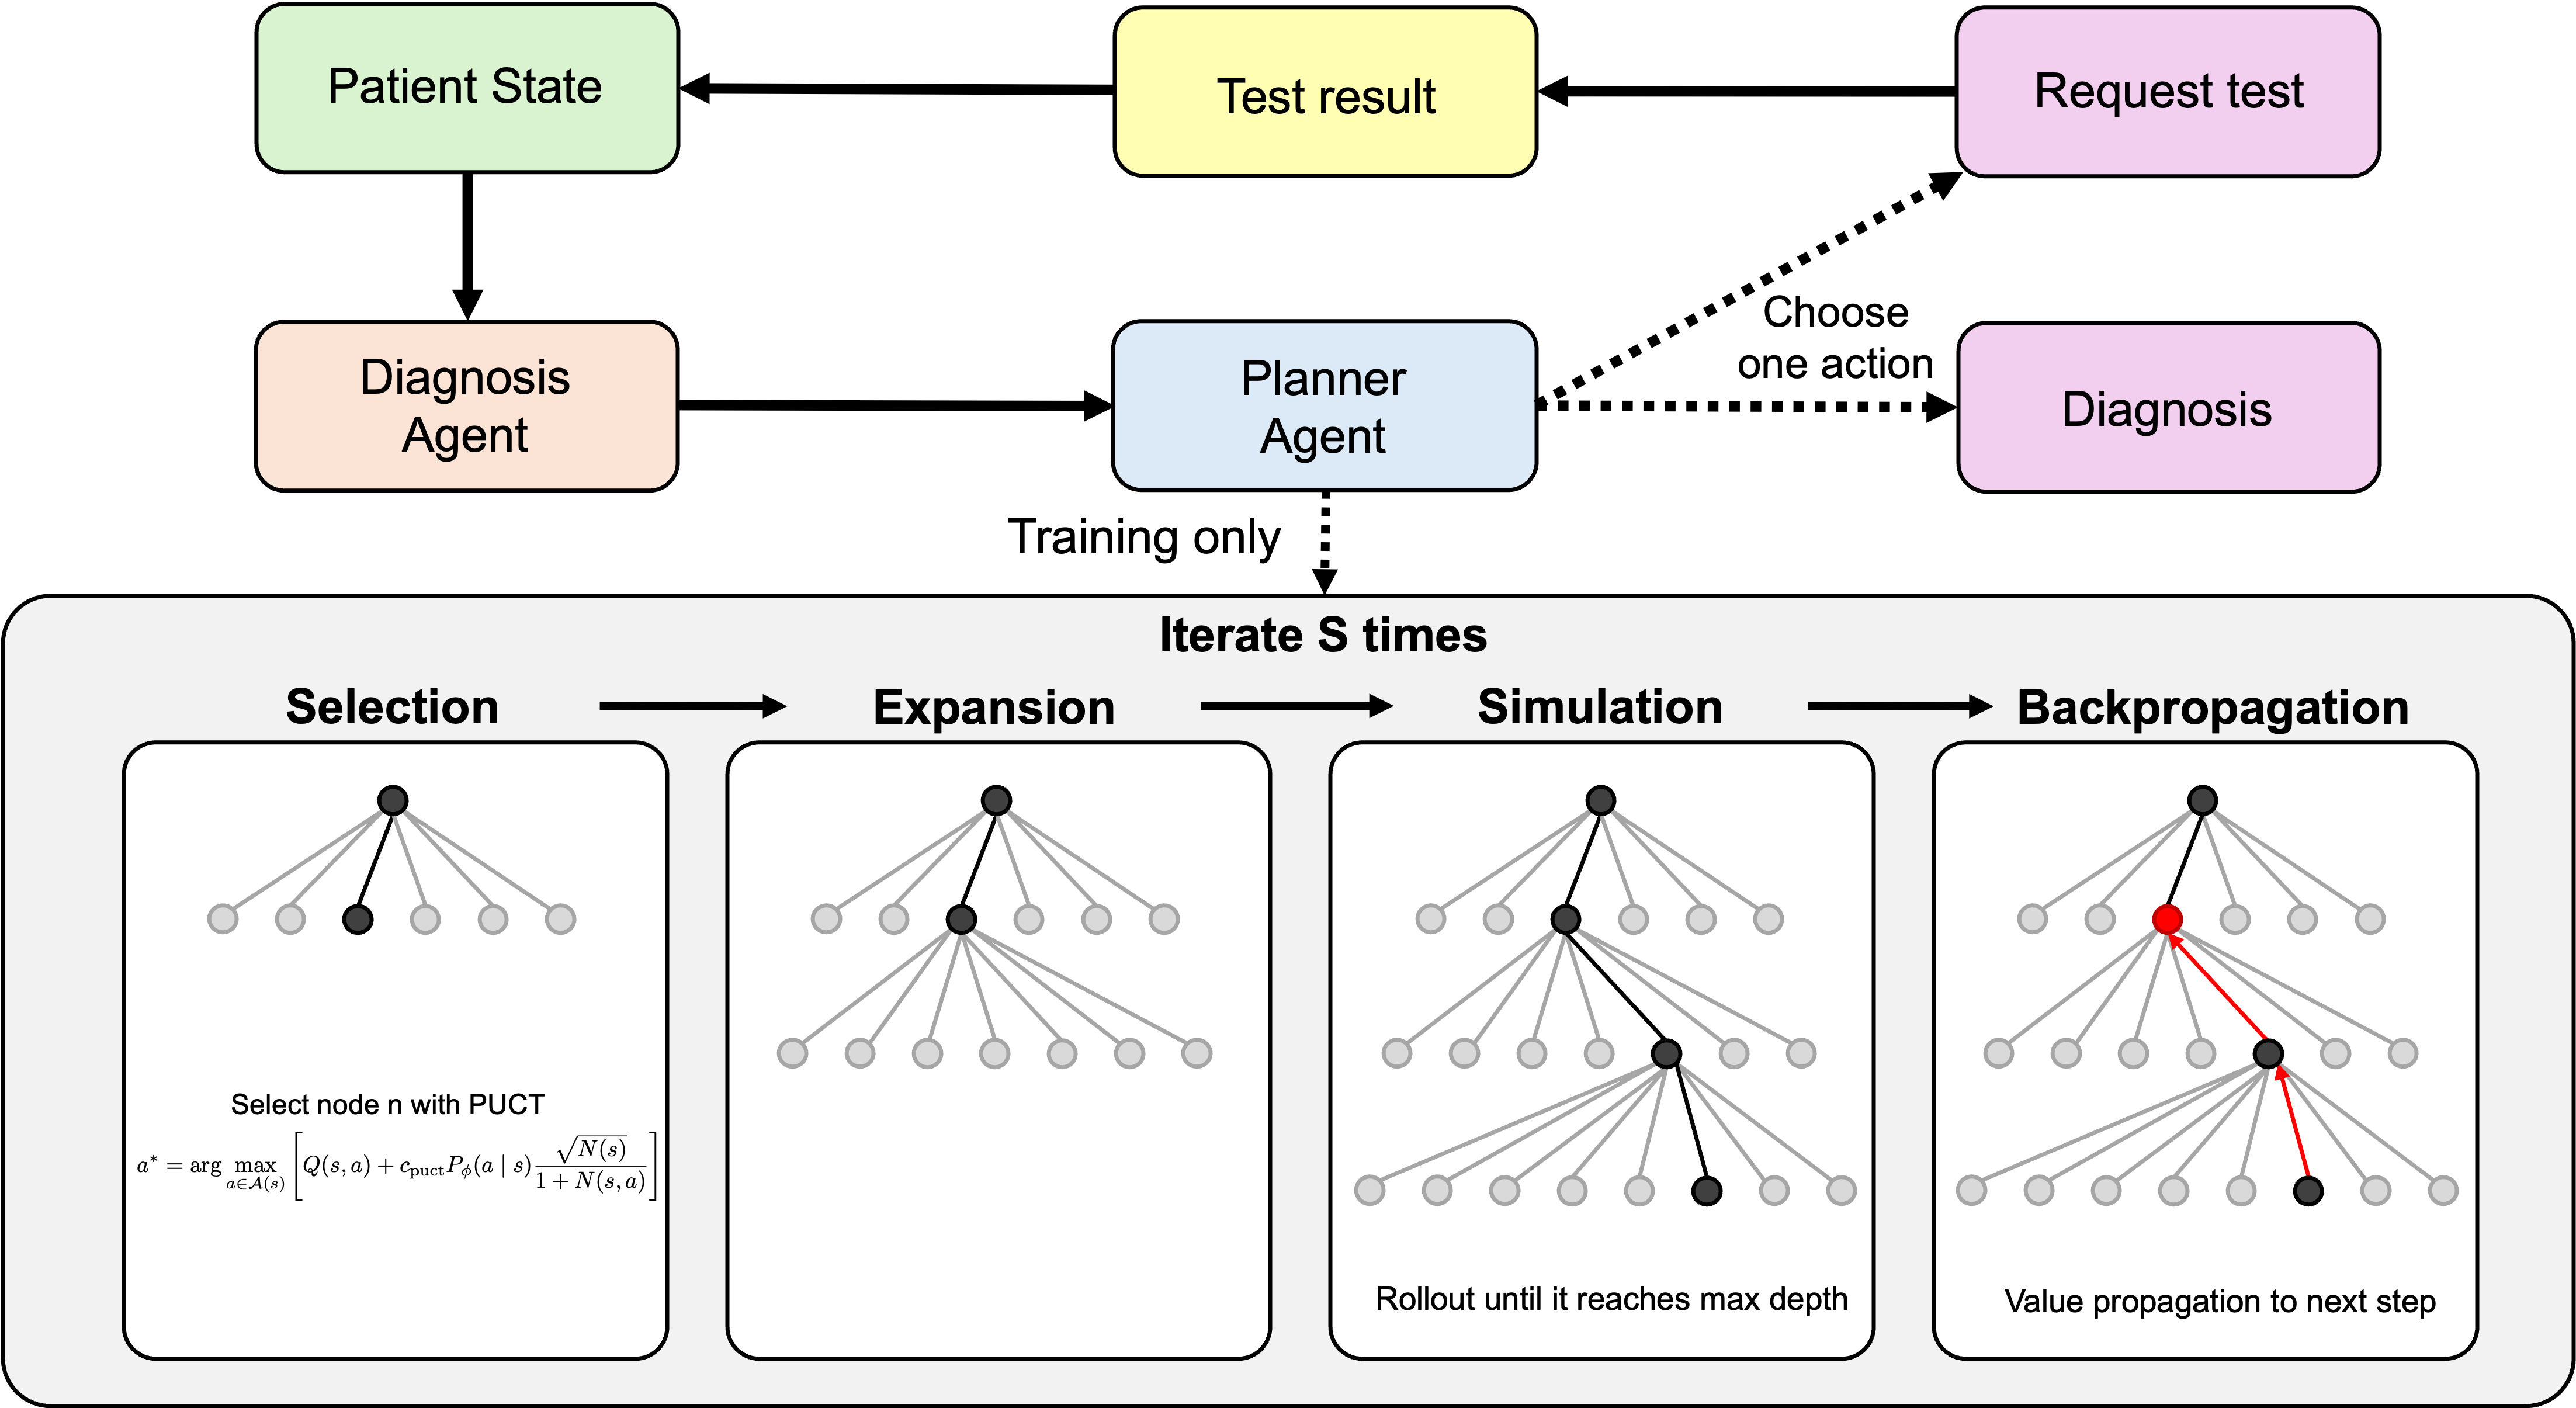
\includegraphics[width=\linewidth,height=0.86\textheight,keepaspectratio]{figures/figure.png}
\end{center}
\end{frame}

\begin{frame}[t]{}
\vspace{-0.25em}
\scriptsize
\setlength{\abovedisplayskip}{1pt}
\setlength{\belowdisplayskip}{1pt}
\begin{columns}[T,onlytextwidth]
\begin{column}{0.45\textwidth}
\textbf{\textcolor{DeepBlue}{Stage 1: Calibrated Diagnostic Agent}}
\vspace{0.18em}

\fcolorbox{GoodGreen}{SoftGreen}{%
\parbox{0.95\linewidth}{\centering
\textbf{Random partial states}\\[-0.1em]
\(s_k=(h_p,\mathcal{T}_{obs}(s_k))\)\\[-0.1em]
\textcolor{gray!70}{sample random observed test subsets}
}}

\vspace{0.12em}
\centering\textcolor{gray!65}{\(\downarrow\)}
\vspace{0.06em}

\fcolorbox{GoodGreen}{SoftGreen}{%
\parbox{0.95\linewidth}{\centering
\textbf{Diagnosis SFT}\\[-0.2em]
\[
\mathcal{L}_{\mathrm{SFT}}
=-\log p_\theta(y_p\mid s_k)
\]
}}

\vspace{0.12em}
\centering\textcolor{gray!65}{\(\downarrow\)}
\vspace{0.06em}

\fcolorbox{GoodGreen}{SoftGreen}{%
\parbox{0.95\linewidth}{\centering
\textbf{Confidence calibration}\\[-0.3em]
\[
R_{\mathrm{conf}}=
\begin{cases}
\log(c_k), & \hat{y}_k=y_p,\\
\log(1-c_k), & \hat{y}_k\neq y_p.
\end{cases}
\]
}}

\vspace{0.34em}
\centering\textcolor{gray!65}{\(\downarrow\)}
\vspace{0.16em}

\fcolorbox{DeepBlue}{SoftBlue}{%
\parbox{0.95\linewidth}{\centering
\textbf{Frozen diagnostic value model}\\[-0.2em]
\(D_\theta(s_k)\rightarrow(\hat{y}_k,c_k)\)\\[-0.4em]
\[
V_D(s_k)=
\begin{cases}
c_k, & \hat{y}_k=y_p,\\
-c_k, & \hat{y}_k\neq y_p.
\end{cases}
\]
}}

\vspace{0.12em}
\begin{center}
\fcolorbox{DeepBlue}{white}{\parbox{0.80\linewidth}{\centering
\textbf{Used in Stage 2}\\
MCTS leaf-state evaluator}}
\end{center}
\end{column}

\begin{column}{0.02\textwidth}
\centering
\textcolor{gray!35}{\rule{0.6pt}{0.80\textheight}}
\end{column}

\begin{column}{0.53\textwidth}
\textbf{\textcolor{DeepBlue}{Stage 2: MCTS-Guided Planner Training}}
\vspace{0.12em}

\fcolorbox{DeepBlue}{white}{\parbox{0.96\linewidth}{
\textbf{1. Current state} \(\;s_k\)
}}

\vspace{0.04em}
\centering\textcolor{gray!65}{\(\downarrow\)}

\fcolorbox{DeepBlue}{white}{\parbox{0.96\linewidth}{
\textbf{2. Planner prior} \(\;\pi_\phi(a\mid s_k),\;a\in\mathcal{A}(s_k)\)
}}

\vspace{0.04em}
\centering\textcolor{gray!65}{\(\downarrow\)}

\fcolorbox{DeepBlue}{white}{\parbox{0.96\linewidth}{
\textbf{3. MCTS lookahead} \((S,H)\), PUCT selection\\[-0.2em]
\[
a=\arg\max_a
\left[
Q(s,a)+c_{\mathrm{puct}}P_\phi(a\mid s)
\frac{\sqrt{N(s)}}{1+N(s,a)}
\right]
\]
}}

\vspace{0.04em}
\centering\textcolor{DeepBlue}{\(\downarrow\)}

\fcolorbox{GoodGreen}{SoftGreen}{\parbox{0.96\linewidth}{
\textbf{4. Leaf evaluation} \quad \fcolorbox{GoodGreen}{white}{Frozen \(D_\theta\)}\\[-0.1em]
\[
G=V_D(s_\ell)-\lambda d
\]
}}

\vspace{0.04em}
\centering\textcolor{DeepBlue}{\(\Downarrow\;\)future value propagation}

\fcolorbox{DeepBlue}{white}{\parbox{0.96\linewidth}{
\textbf{5. Q backup}\\[-0.2em]
\[
Q(s,a)=\frac{1}{N(s,a)}\sum_{i:(s,a)\in\tau_i}G_i
\]
}}

\vspace{0.04em}
\centering\textcolor{gray!65}{\(\downarrow\)}

\fcolorbox{DeepBlue}{white}{\parbox{0.96\linewidth}{
\textbf{6. Planner distillation}\\[-0.2em]
\[
p_{\mathrm{MCTS}}(a\mid s_k)=\mathrm{softmax}(Q(s_k,a)/\tau)
\]
\[
\mathcal{L}_{planner}
=-\sum_a p_{\mathrm{MCTS}}(a\mid s_k)\log\pi_\phi(a\mid s_k)
\]
}}

\vspace{0.04em}
\centering\textcolor{gray!65}{\(\downarrow\)}

\fcolorbox{DeepBlue}{white}{\parbox{0.96\linewidth}{
\textbf{7. Limited commitment} execute one action; repeat.
}}
\end{column}
\end{columns}
\end{frame}

\begin{frame}{Performance Comparison}
\vspace{-0.2em}
\begin{center}
\scriptsize
\resizebox{\linewidth}{!}{
\begin{tabular}{lccccccccc}
\toprule
\multirow{2}{*}{\textbf{Method}} &
\multicolumn{6}{c}{\textbf{Accuracy}} &
\multicolumn{2}{c}{\textbf{F1-Score}} &
\multirow{2}{*}{\textbf{Mean Tests}} \\
\cmidrule(lr){2-7}\cmidrule(lr){8-9}
& \textbf{Append.} & \textbf{Chole.} & \textbf{Divert.} & \textbf{Pancr.} & \textbf{Mean} & \textbf{Acc.} & \textbf{Micro} & \textbf{Macro} & \\
\midrule
OASST* & 82.0 & 48.0 & 45.5 & 44.1 & 54.9 & -- & -- & -- & -- \\
ReAct & 77.1 & 66.2 & 60.0 & 31.5 & 58.7 & 62.1 & 69.8 & 64.4 & 3.03 \\
LA-CDM (3B) & 80.2 & 73.8 & 56.0 & 51.9 & 65.5 & 69.6 & 75.9 & 72.1 & 1.37 \\
\midrule
SFT-all & 95.8 & 83.1 & 100.0 & 83.3 & 90.6 & 90.0 & 90.0 & 89.0 & All \\
Stage1 (LA-CDM prompt) & 93.8 & 72.3 & 92.0 & 66.7 & 81.0 & 81.5 & 81.5 & 79.3 & -- \\
Ours (MCTS, H=3, S=8) & 93.8 & 83.1 & 84.0 & 81.5 & 85.6 & 87.1 & 87.1 & 85.5 & 7.08 \\
\bottomrule
\end{tabular}
}
\end{center}

\vspace{-0.15em}
\scriptsize
\textcolor{gray!75}{*OASST results are taken from Hager et al. (2024), evaluated under the original MIMIC-CDM open-ended framework with a different test setting.}

\vspace{0.25em}
\small
\begin{center}
\begin{minipage}{0.94\linewidth}
현재 MCTS \(H=3, S=8\) 설정은 mean class-wise accuracy 85.6, overall accuracy 87.1로 baseline보다 크게 높다. 다만 평균 검사 수가 7.08로 많아, 다음 단계에서는 test-cost penalty나 stop calibration을 통해 성능을 유지하면서 검사 수를 줄이는 것이 핵심이다.
\end{minipage}
\end{center}
\end{frame}

\begin{frame}{현재 문제: Stage 1 Confidence Calibration}
\vspace{0.05em}
\begin{center}
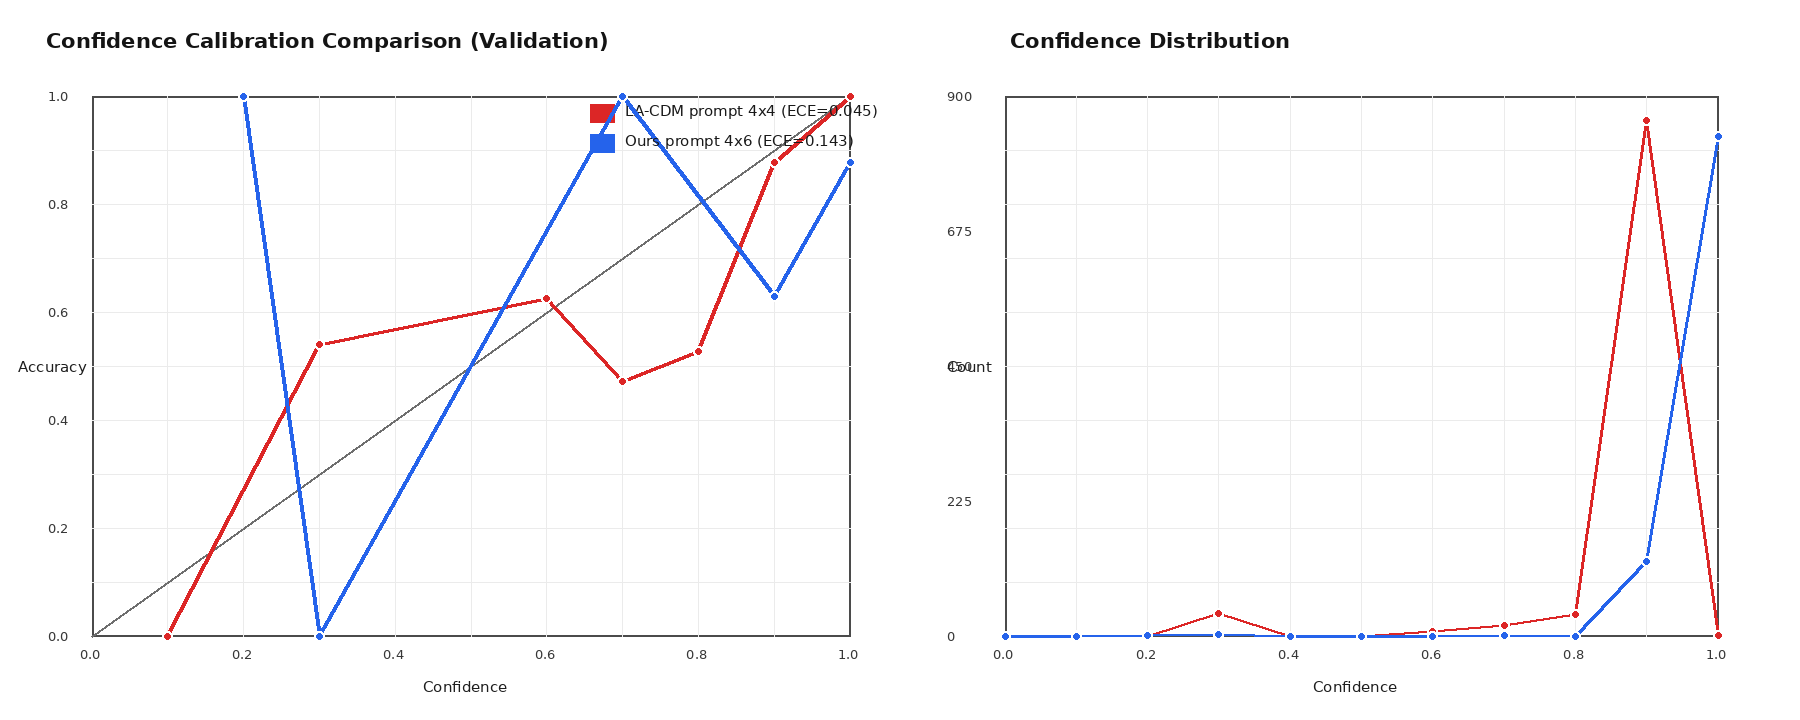
\includegraphics[width=\linewidth,height=0.68\textheight,keepaspectratio]{figures/confcal.png}

\vspace{0.15em}
\small
\textcolor{DeepBlue}{현재 confidence가 일부 높은 bin에 몰려 있어, stop decision에 사용하기 전 calibration 안정화가 필요하다.}
\end{center}
\end{frame}

\begin{frame}{다음 작업}
\vspace{0.4em}
\begin{block}{1순위: Diagnostic Agent Calibration}
\small
프롬프트를 바꿔가며 partial state에서 안정적인 diagnosis와 confidence를 뽑는 설정을 찾는다. 핵심 지표는 accuracy, ECE, none/unknown fraction이다.
\end{block}

\vspace{0.35em}
\begin{block}{2순위: Planner Search Setting}
\small
Planner에서 horizon \(H\), simulation count \(S\), 그리고 stop criterion을 바꿔가며 성능과 평균 검사 수의 trade-off를 확인한다.
\end{block}
\end{frame}

\begin{frame}[plain]
\begin{center}
\vspace{1.6cm}
{\Huge\bfseries\textcolor{DeepBlue}{Next Direction}}\\[1.0em]
{\Large Single-Agent Clinical Decision Making}\\[0.8em]
{\normalsize 진단, 불확실성, 검사 선택을 하나의 likelihood space에서 학습}
\end{center}
\end{frame}

\begin{frame}{기존 방법의 한계}
\vspace{0.15em}
\begin{columns}[T,onlytextwidth]
\begin{column}{0.44\textwidth}
\begin{block}{Two-agent: 진단과 검사 선택의 단절}
\small
임상에서 검사는 단순히 1순위 진단을 확인하는 행동이 아니라, 서로 헷갈리는 진단 후보들을 구분하기 위한 행동이다.

\vspace{0.1em}
\begin{center}
\textcolor{DeepBlue}{\(\Downarrow\)}
\end{center}
\vspace{-0.2em}
다음 검사는 별도의 planner가 독립적으로 고르는 것이 아니라, 현재 진단의 불확실성에서 직접 결정되어야 한다.

\vspace{0.25em}
\scriptsize
\begin{itemize}
  \item 췌장염 vs. 담낭염이 헷갈리니 \(\rightarrow\) lab / image로 판별
  \item 충수염 vs. 게실염이 헷갈리니 \(\rightarrow\) image / physical로 판별
\end{itemize}
\end{block}
\end{column}

\begin{column}{0.08\textwidth}
\vspace{3.3em}
\begin{center}
{\Large\textcolor{DeepBlue}{\(\Longrightarrow\)}}\\[-0.1em]
{\tiny\textcolor{DeepBlue}{interface}}
\end{center}
\end{column}

\begin{column}{0.44\textwidth}
\begin{block}{Top-1 confidence로 감별 상태가 축약됨}
\small
Planner가 받는 신호가 top-1 진단과 verbal confidence로 축약되면, 어떤 질환들이 서로 얼마나 가까운지에 대한 정보가 사라진다.

\vspace{0.35em}
\centering
\fcolorbox{LineGray}{white}{Hypothesis: A}\\[0.2em]
\fcolorbox{LineGray}{white}{Confidence: 8}\\[0.35em]
\(\not\Rightarrow\) \(A\) vs. \(B,C,D\) separability
\end{block}
\end{column}
\end{columns}

\vspace{1.15em}
\begin{center}
\begin{tikzpicture}[node distance=0.8cm, scale=1.02, transform shape]
\node[greenbox, minimum width=3.0cm] (da) {Diagnosis Agent\\\scriptsize reads patient state};
\node[yellowbox, minimum width=2.9cm, right=1.6cm of da] (msg) {Interface\\\scriptsize Hypothesis: A\\\scriptsize Confidence: 8};
\node[bluebox, minimum width=3.0cm, right=1.6cm of msg] (pa) {Planner Agent\\\scriptsize selects next test};
\draw[arrow] (da) -- (msg);
\draw[arrow] (msg) -- (pa);
\node[font=\scriptsize, text=red!75!black, align=center, below=0.28cm of msg]
{정보 손실\\\(p(A),p(B),p(C),p(D)\), separability};
\end{tikzpicture}
\end{center}
\end{frame}

\begin{frame}{Confidence to Separability}
\vspace{0.05em}
\small
\begin{block}{핵심 직관}
\small
순차 진단에서 confidence는 ``가장 그럴듯한 질환 하나''의 점수가 아니라,
\textbf{4개 감별진단 토큰의 분포가 얼마나 벌어져 있는가}로 판단해야 한다.
\end{block}

\vspace{0.15em}
\begin{center}
\begin{tikzpicture}[x=1cm,y=1cm]
\node[bluebox, minimum width=2.4cm] (state) at (0,1.9) {Patient state\\\(s_k\)};
\node[greenbox, minimum width=3.1cm] (llm) at (3.1,1.9) {Same LLM\\next-token logits};
\draw[arrow] (state) -- (llm);

\draw[LineGray, thick, ->] (5.0,0.2) -- (10.9,0.2) node[right, font=\scriptsize] {disease token};
\draw[LineGray, thick, ->] (5.0,0.2) -- (5.0,3.0) node[above, font=\scriptsize] {prob.};

\foreach \x/\h/\tok/\logit/\prob/\col in {
5.55/2.35/App/\(z_{\mathrm{app}}\)/\(p=.55\)/SoftBlue,
6.95/2.05/Chol/\(z_{\mathrm{chol}}\)/\(p=.32\)/SoftGreen,
8.35/0.85/Div/\(z_{\mathrm{div}}\)/\(p=.08\)/SoftYellow,
9.75/0.55/Pan/\(z_{\mathrm{pan}}\)/\(p=.05\)/white}
{
  \draw[fill=\col, draw=DeepBlue, thick] (\x,0.2) rectangle +(0.72,\h);
  \node[font=\scriptsize, align=center] at (\x+0.36,-0.28) {\tok\\[-0.1em]\tiny \prob};
  \node[font=\scriptsize, align=center] at (\x+0.36,\h+0.55) {\logit};
}

\node[font=\scriptsize, align=center, text=DeepBlue] at (7.7,3.35)
{4개 질환 토큰의 로짓을 softmax하여\\하나의 이산 확률분포로 해석};
\draw[greenarrow] (llm.east) -- (5.0,1.9);
\end{tikzpicture}
\end{center}

\vspace{0.05em}
\begin{columns}[T,onlytextwidth]
\begin{column}{0.48\textwidth}
\begin{block}{기존 confidence}
\scriptsize
\[
\text{Diagnosis: App,\quad Confidence: 8}
\]
\vspace{-0.3em}
\begin{itemize}
  \item top-1 진단 하나만 요약
  \item 다른 질환과 얼마나 가까운지 손실
\end{itemize}
\end{block}
\end{column}

\begin{column}{0.48\textwidth}
\begin{block}{Diagnostic margin}
\scriptsize
\[
m(s_k)=z_{(1)}(s_k)-z_{(2)}(s_k)
\]
\vspace{-0.3em}
\begin{itemize}
  \item margin이 크면 진단 가능
  \item margin이 작으면 추가 검사 필요
\end{itemize}
\end{block}
\end{column}
\end{columns}
\end{frame}

\begin{frame}{Special Token으로 의사결정 분해}
\vspace{0.05em}
\small
\begin{block}{핵심 구조}
\small
같은 LLM이 먼저 special token으로 \textbf{지금 진단할지} 또는 \textbf{추가 검사를 요청할지}를 결정하고,
선택된 phase 안에서만 후보 토큰을 scoring한다.
\end{block}

\vspace{0.25em}
\begin{center}
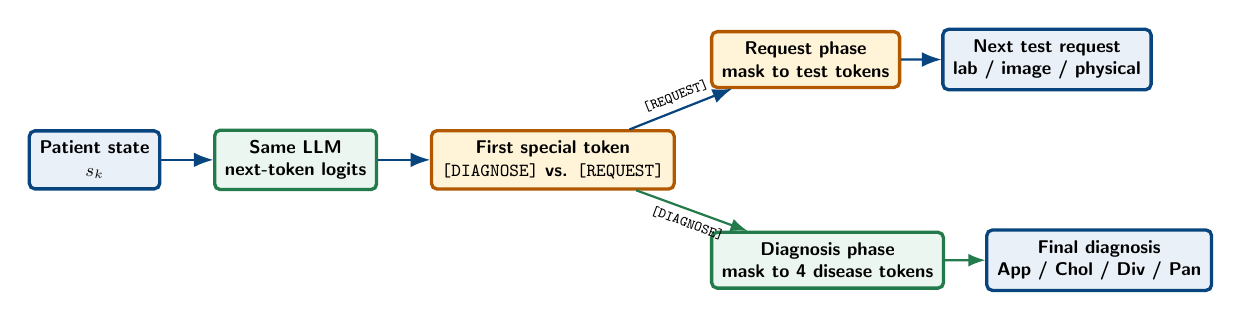
\begin{tikzpicture}[node distance=0.85cm, scale=0.74, transform shape]
\node[bluebox, minimum width=2.2cm] (state) {Patient state\\\(s_k\)};
\node[greenbox, minimum width=2.7cm, right=0.9cm of state] (llm) {Same LLM\\next-token logits};
\node[yellowbox, minimum width=3.0cm, right=0.9cm of llm] (gate) {First special token\\\(\texttt{[DIAGNOSE]}\) vs. \(\texttt{[REQUEST]}\)};

\node[greenbox, minimum width=3.0cm, below right=0.7cm and 0.6cm of gate] (dx) {Diagnosis phase\\mask to 4 disease tokens};
\node[yellowbox, minimum width=3.0cm, above right=0.7cm and 0.6cm of gate] (req) {Request phase\\mask to test tokens};

\node[bluebox, minimum width=2.7cm, right=0.7cm of dx] (dxout) {Final diagnosis\\App / Chol / Div / Pan};
\node[bluebox, minimum width=2.7cm, right=0.7cm of req] (reqout) {Next test request\\lab / image / physical};

\draw[arrow] (state) -- (llm);
\draw[arrow] (llm) -- (gate);
\draw[greenarrow] (gate) -- node[below, sloped, font=\scriptsize] {\(\texttt{[DIAGNOSE]}\)} (dx);
\draw[arrow] (gate) -- node[above, sloped, font=\scriptsize] {\(\texttt{[REQUEST]}\)} (req);
\draw[greenarrow] (dx) -- (dxout);
\draw[arrow] (req) -- (reqout);
\end{tikzpicture}
\end{center}

\vspace{0.1em}
\begin{columns}[T,onlytextwidth]
\begin{column}{0.49\textwidth}
\begin{block}{왜 필요한가}
\scriptsize
\begin{itemize}
  \item 진단/검사 선택을 한 softmax에 섞지 않음
  \item stop decision을 special token 확률로 표현
  \item phase별 후보만 남겨 action space를 줄임
\end{itemize}
\end{block}
\end{column}

\begin{column}{0.49\textwidth}
\begin{block}{추론 흐름}
\scriptsize
\[
p_\theta(g\mid s_k),\quad g\in\{\texttt{[DIAGNOSE]},\texttt{[REQUEST]}\}
\]
\vspace{-0.3em}
\[
p_\theta(a\mid s_k,g)\quad \text{with phase-specific masking}
\]
\end{block}
\end{column}
\end{columns}
\end{frame}

\end{document}

\begin{frame}{핵심 질문}
\vspace{0.3em}
\begin{block}{목표}
\small
현재 환자 state에서 다음 검사를 선택할 때, 단기적으로 그럴듯한 검사가 아니라
\textbf{\(n\)-step 이후 진단 상태를 가장 많이 개선하는 검사}를 학습하고 싶다.
\end{block}

\vspace{0.5em}
\begin{center}
\begin{tikzpicture}[scale=0.95, transform shape]
\node[state] (s) at (0,0) {현재 state\\\(s_t\)};
\node[action] (a1) at (2.0,1.1) {Blood};
\node[action] (a2) at (2.0,0) {CT};
\node[action] (a3) at (2.0,-1.1) {Stop};
\node[value] (v1) at (5.0,1.1) {미래 \(V=0.58\)};
\node[value] (v2) at (5.0,0) {미래 \(V=0.83\)};
\node[value] (v3) at (5.0,-1.1) {현재 \(V=0.49\)};
\node[greenbox, minimum width=2.4cm] (best) at (7.6,0) {CT 선택};
\draw[arrow] (s) -- (a1);
\draw[arrow] (s) -- (a2);
\draw[arrow] (s) -- (a3);
\draw[grayarrow] (a1) -- (v1);
\draw[arrow] (a2) -- (v2);
\draw[grayarrow] (a3) -- (v3);
\draw[greenarrow] (v2) -- (best);
\end{tikzpicture}
\end{center}

\vspace{0.25em}
\begin{alertblock}{핵심 관점}
\small
검사 선택은 reasoning 문제가 아니라 planning 문제다. 현재 action의 가치는 이후 검사들과의 조합, 중복성, stop timing에 의해 결정된다.
\end{alertblock}
\end{frame}

\begin{frame}{기존 방향: LA-CDM의 보상 구조}
\vspace{0.15em}
\begin{block}{LA-CDM의 강점}
\small
LA-CDM도 exploration--exploitation 기반의 trial-and-error를 수행한다. 여러 진단 trajectory를 생성하고, 최종 진단 성공과 검사 비용을 통해 좋은 trajectory를 강화한다.
\end{block}

\vspace{0.2em}
\begin{center}
\begin{tikzpicture}[scale=0.9, transform shape]
\node[state] (s0) at (0,0) {\(s_0\)};
\node[state] (s1) at (1.85,0) {\(s_1\)};
\node[state] (s2) at (3.70,0) {\(s_2\)};
\node[state] (s3) at (5.55,0) {\(s_3\)};
\node[state] (sf) at (7.40,0) {진단};
\node[action] at (0.92,0.55) {검사 A};
\node[action] at (2.77,0.55) {검사 B};
\node[action] at (4.62,0.55) {검사 C};
\node[action] at (6.47,0.55) {Stop};
\draw[arrow] (s0) -- (s1);
\draw[arrow] (s1) -- (s2);
\draw[arrow] (s2) -- (s3);
\draw[arrow] (s3) -- (sf);
\draw[draw=WarnRed, very thick, rounded corners=7pt]
  (0.2,-0.46) -- (0.2,-0.85) -- (7.30,-0.85) -- (7.30,-0.46);
\node[redbox, minimum width=6.9cm] at (3.75,-1.30)
  {최종 진단 성공/비용 기반 trajectory reward};
\end{tikzpicture}
\end{center}

\vspace{0.15em}
\begin{alertblock}{한계}
\small
최종 trajectory가 좋더라도, 그 안의 모든 검사가 실제로 좋은 것은 아니다.
즉, \textbf{어떤 검사 action이 진단 개선에 기여했는지}에 대한 step-level supervision이 약하다.
\end{alertblock}
\end{frame}

\begin{frame}{ORM vs PRM 관점}
\vspace{0.2em}
\begin{columns}[T,onlytextwidth]
\begin{column}{0.48\textwidth}
\begin{center}
\begin{tikzpicture}
\node[redbox, minimum width=0.95\linewidth] {
ORM-like\\
\small 최종 결과 중심 보상
};
\end{tikzpicture}
\end{center}
\vspace{0.25em}
\scriptsize
\begin{itemize}
  \item 최종 진단이 맞았는지 평가
  \item 검사 비용을 포함한 trajectory-level reward
  \item sparse signal
  \item action-level credit assignment가 약함
\end{itemize}
\end{column}
\begin{column}{0.48\textwidth}
\begin{center}
\begin{tikzpicture}
\node[greenbox, minimum width=0.95\linewidth] {
PRM-like\\
\small 과정/행동 단위 value
};
\end{tikzpicture}
\end{center}
\vspace{0.25em}
\scriptsize
\begin{itemize}
  \item 현재 state-action의 미래 진단 가치 평가
  \item leaf value를 현재 action으로 backpropagation
  \item dense signal
  \item 검사별 기여도 분리 가능
\end{itemize}
\end{column}
\end{columns}

\vspace{0.45em}
\begin{block}{정리}
\small
LA-CDM은 ORM-like terminal/trajectory reward에 가깝다. 제안 방향은 MCTS lookahead를 통해 PRM-like dense state-action value를 만들고, 이를 Planner 학습 신호로 사용한다.
\end{block}
\end{frame}

\begin{frame}{왜 Planning인가?}
\vspace{0.2em}
\begin{block}{Why Reasoning Fails to Plan의 관점}
\small
LLM의 step-wise reasoning은 현재 step에서 그럴듯한 선택을 잘 할 수 있지만, 장기 horizon에서는 local greedy decision에 머무르기 쉽다. Planning에는 다음 세 가지가 필요하다.
\end{block}

\vspace{0.25em}
\begin{center}

\begin{tikzpicture}[scale=0.95, transform shape]
\node[bluebox, minimum width=3.0cm] (l) at (0,0) {Explicit\\Lookahead};
\node[greenbox, minimum width=3.0cm] (b) at (3.8,0) {Backward Value\\Propagation};
\node[purplebox, minimum width=3.0cm] (c) at (7.6,0) {Limited\\Commitment};
\draw[arrow] (l) -- (b);
\draw[arrow] (b) -- (c);
\end{tikzpicture}
\end{center}

\vspace{0.35em}
\scriptsize
\begin{itemize}
  \item \term{Explicit lookahead}: 후보 검사를 \(n\)-step까지 가상 진행하고 이후 진단 상태를 평가한다.
  \item \term{Backward value propagation}: 미래 진단 value를 현재 action의 가치로 되돌린다.
  \item \term{Limited commitment}: 전체 검사 sequence를 한 번에 실행하지 않고, 한 action만 선택한 뒤 다음 state에서 다시 planning한다.
\end{itemize}
\end{frame}

\begin{frame}{제안 구조: 두 에이전트}
\vspace{0.15em}
\begin{center}
\begin{tikzpicture}[scale=0.96, transform shape]
\draw[gray!40, line width=0.8pt] (4.55,-1.95) -- (4.55,2.05);

\node[font=\bfseries\small, text=DeepBlue] at (2.0,1.65) {Stage 1};
\node[greenbox, minimum width=3.6cm, minimum height=1.45cm] (diag) at (2.0,0.45)
  {Diagnosis +\\Confidence Agent};
\node[align=center, font=\scriptsize, text=TextGray, text width=3.7cm] at (2.0,-0.95)
  {부분 evidence state마다\\진단과 calibrated confidence 예측\\수렴 후 freeze};

\node[font=\bfseries\small, text=DeepBlue] at (7.1,1.65) {Stage 2};
\node[bluebox, minimum width=3.6cm, minimum height=1.45cm] (plan) at (7.1,0.45)
  {Planner Agent +\\MCTS Lookahead};
\node[align=center, font=\scriptsize, text=TextGray, text width=3.8cm] at (7.1,-0.95)
  {MCTS가 만든 best action을\\pseudo-label로 사용해\\Planner를 지도학습};

\draw[greenarrow, bend left=12] (diag.east) to node[above, font=\scriptsize] {leaf 평가} (plan.west);
\end{tikzpicture}
\end{center}

\vspace{0.2em}
\begin{block}{핵심}
\small
Diagnosis + Confidence Agent는 value evaluator 역할을 하고, Planner Agent는 MCTS teacher가 선택한 action을 학습하는 student 역할을 한다.
\end{block}
\end{frame}

\begin{frame}{Stage 1: Diagnosis + Confidence Agent}
\vspace{0.15em}
\begin{block}{학습 목표}
\small
다양한 부분 환자 상태에서 진단을 맞추고, 그 진단에 대한 confidence를 calibration한다.
\end{block}

\vspace{0.2em}
\begin{center}
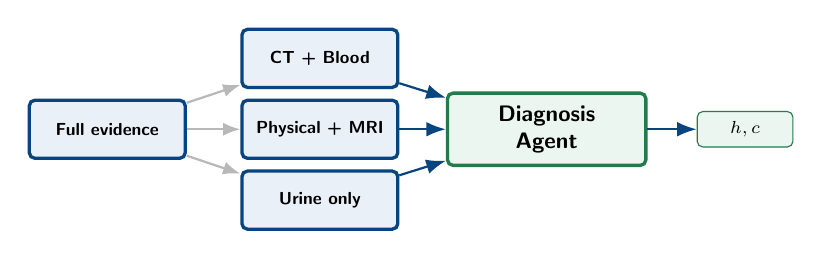
\begin{tikzpicture}[scale=0.9, transform shape]
\node[state, minimum width=2.2cm] (full) at (0,0) {Full evidence};
\node[state, minimum width=2.2cm] (p1) at (3.0,1.0) {CT + Blood};
\node[state, minimum width=2.2cm] (p2) at (3.0,0) {Physical + MRI};
\node[state, minimum width=2.2cm] (p3) at (3.0,-1.0) {Urine only};
\node[greenbox, minimum width=2.8cm] (agent) at (6.2,0) {Diagnosis\\Agent};
\node[value] (out) at (9.0,0) {\(h, c\)};
\draw[grayarrow] (full) -- (p1);
\draw[grayarrow] (full) -- (p2);
\draw[grayarrow] (full) -- (p3);
\draw[arrow] (p1) -- (agent);
\draw[arrow] (p2) -- (agent);
\draw[arrow] (p3) -- (agent);
\draw[arrow] (agent) -- (out);
\end{tikzpicture}
\end{center}

\vspace{0.2em}
\scriptsize
\begin{itemize}
  \item 검사 결과를 일부 drop하여 다양한 partial state 생성
  \item Drop률을 \(0.1 \rightarrow 0.8/0.9\)로 올리는 curriculum learning
  \item 진단 정확도와 confidence calibration을 함께 개선
  \item 수렴 후 freeze하여 Planner 학습의 evaluator로 사용
\end{itemize}
\end{frame}

\begin{frame}{Stage 2: MCTS Lookahead}
\vspace{0.15em}
\begin{center}
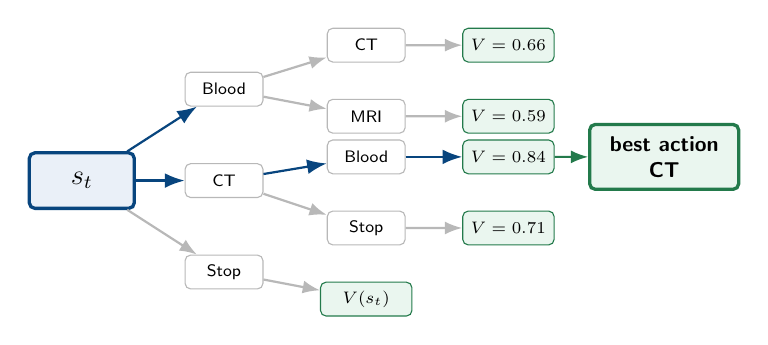
\begin{tikzpicture}[scale=0.86, transform shape]
\node[state, font=\large\bfseries] (root) at (0,0) {\(s_t\)};

\node[action] (a1) at (2.1,1.35) {Blood};
\node[action] (a2) at (2.1,0) {CT};
\node[action] (a3) at (2.1,-1.35) {Stop};

\node[action] (b11) at (4.2,2.0) {CT};
\node[action] (b12) at (4.2,0.95) {MRI};
\node[action] (b21) at (4.2,0.35) {Blood};
\node[action] (b22) at (4.2,-0.70) {Stop};
\node[value] (vstop) at (4.2,-1.75) {\(V(s_t)\)};

\node[value] (v11) at (6.3,2.0) {\(V=0.66\)};
\node[value] (v12) at (6.3,0.95) {\(V=0.59\)};
\node[value] (v21) at (6.3,0.35) {\(V=0.84\)};
\node[value] (v22) at (6.3,-0.70) {\(V=0.71\)};

\node[greenbox, minimum width=2.2cm] (best) at (8.6,0.35) {best action\\CT};

\draw[arrow] (root) -- (a1);
\draw[arrow] (root) -- (a2);
\draw[grayarrow] (root) -- (a3);
\draw[grayarrow] (a1) -- (b11);
\draw[grayarrow] (a1) -- (b12);
\draw[arrow] (a2) -- (b21);
\draw[grayarrow] (a2) -- (b22);
\draw[grayarrow] (a3) -- (vstop);
\draw[grayarrow] (b11) -- (v11);
\draw[grayarrow] (b12) -- (v12);
\draw[arrow] (b21) -- (v21);
\draw[grayarrow] (b22) -- (v22);
\draw[greenarrow] (v21) -- (best);
\end{tikzpicture}
\end{center}

\vspace{0.1em}
\begin{block}{절차}
\small
현재 state를 root로 두고, 가능한 검사 12종 + Stop을 branch로 확장한다. Leaf state는 freeze된 Diagnosis + Confidence Agent로 평가하고, leaf value를 root action의 \(Q\)-value로 backpropagation한다.
\end{block}
\end{frame}

\begin{frame}{MCTS에서 만드는 학습 신호}
\vspace{0.1em}
\begin{block}{Leaf 평가}
\small
\[
D_\theta(s_{\mathrm{leaf}}) \rightarrow (h_{\mathrm{leaf}}, c_{\mathrm{leaf}})
\]
\[
R_{\mathrm{leaf}} =
\begin{cases}
c_{\mathrm{leaf}}, & h_{\mathrm{leaf}} = y \\
-c_{\mathrm{leaf}}, & h_{\mathrm{leaf}} \neq y \\
0, & \text{invalid state}
\end{cases}
\qquad
G_{\mathrm{leaf}} = \gamma^d R_{\mathrm{leaf}}
\]
\end{block}

\vspace{0.25em}
\begin{center}
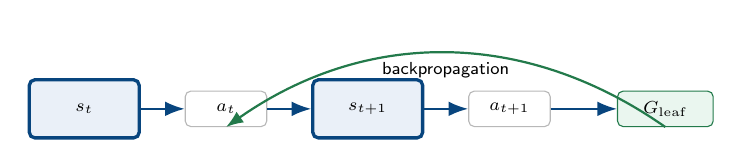
\begin{tikzpicture}[scale=0.9, transform shape]
\node[state] (s) at (0,0) {\(s_t\)};
\node[action] (a) at (2.0,0) {\(a_t\)};
\node[state] (s1) at (4.0,0) {\(s_{t+1}\)};
\node[action] (a2) at (6.0,0) {\(a_{t+1}\)};
\node[value] (leaf) at (8.2,0) {\(G_{\mathrm{leaf}}\)};
\draw[arrow] (s) -- (a);
\draw[arrow] (a) -- (s1);
\draw[arrow] (s1) -- (a2);
\draw[arrow] (a2) -- (leaf);
\draw[greenarrow, bend right=35] (leaf.south) to node[below, font=\scriptsize] {backpropagation} (a.south);
\end{tikzpicture}
\end{center}

\vspace{0.15em}
\begin{alertblock}{핵심}
\small
최종 trajectory reward만 주는 것이 아니라, 미래 진단 value를 현재 action의 \(Q(s_t,a_t)\)로 되돌려 \textbf{dense state-action supervision}을 만든다.
\end{alertblock}
\end{frame}

\begin{frame}{Planner 학습}
\vspace{0.15em}
\begin{block}{MCTS teacher \(\rightarrow\) Planner student}
\small
각 환자 state에서 MCTS가 root action별 \(Q\)-value를 계산한다. 가장 높은 \(Q\)-value를 가진 action을 pseudo-label로 사용해 Planner를 지도학습한다.
\end{block}

\vspace{0.3em}
\begin{center}
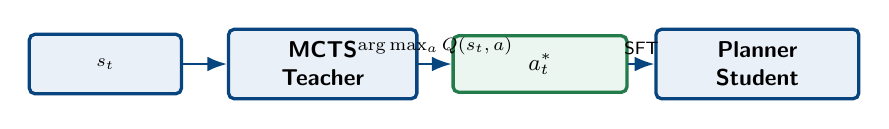
\begin{tikzpicture}[scale=0.92, transform shape]
\node[state, minimum width=2.1cm] (s) at (0,0) {\(s_t\)};
\node[bluebox, minimum width=2.6cm] (mcts) at (3.0,0) {MCTS\\Teacher};
\node[greenbox, minimum width=2.4cm] (label) at (6.0,0) {\(a_t^\ast\)};
\node[bluebox, minimum width=2.8cm] (planner) at (9.0,0) {Planner\\Student};
\draw[arrow] (s) -- (mcts);
\draw[arrow] (mcts) -- node[above, font=\scriptsize] {\(\arg\max_a Q(s_t,a)\)} (label);
\draw[arrow] (label) -- node[above, font=\scriptsize] {SFT} (planner);
\end{tikzpicture}
\end{center}

\vspace{0.25em}
\[
\mathcal{L}_{\mathrm{planner}}
= -\log \pi_\phi(a_t^\ast \mid s_t, h_t, c_t, A_t)
\]

\vspace{0.1em}
\scriptsize
\begin{itemize}
  \item \(A_t\): 현재 가능한 검사 action set + Stop
  \item 학습 시에는 MCTS를 많이 사용하고, 추론 시에는 Planner가 바로 action 선택
  \item 즉, expensive search를 cheap policy로 distillation하는 구조
\end{itemize}
\end{frame}

\begin{frame}{LA-CDM 대비 부각할 점}
\vspace{0.1em}
\begin{center}
\scriptsize
\begin{tabularx}{\textwidth}{p{0.23\textwidth}XX}
\toprule
 & \textbf{LA-CDM} & \textbf{제안 방법} \\
\midrule
Reward granularity &
최종 진단/비용 중심의 trajectory reward &
미래 진단 value를 state-action으로 backpropagation \\
\addlinespace
ORM/PRM 관점 &
ORM-like terminal feedback &
PRM-like dense process/value supervision \\
\addlinespace
Exploration &
trial-and-error는 가능하지만 action별 기여도 분리가 약함 &
MCTS로 promising action을 더 깊게 탐색하고 value를 재사용 \\
\addlinespace
검사 조합효과 &
최종 trajectory 성공에 간접 반영 &
\(n\)-step lookahead로 검사 간 complementarity와 redundancy를 직접 반영 \\
\addlinespace
Stop decision &
최종 보상으로 간접 학습 &
현재 stop value와 추가 검사 future value를 직접 비교 \\
\bottomrule
\end{tabularx}
\end{center}

\vspace{0.25em}
\begin{block}{주장}
\small
두 방법 모두 trial-and-error를 하지만, 제안 방법은 future diagnostic outcome을 dense한 state-action value로 변환하므로 exploration이 더 효율적이고 action-level credit assignment가 명확하다.
\end{block}
\end{frame}

\begin{frame}{우려사항과 검증 포인트}
\vspace{0.1em}
\begin{columns}[T,onlytextwidth]
\begin{column}{0.48\textwidth}
\begin{center}
\begin{tikzpicture}
\node[redbox, minimum width=0.95\linewidth] {
우려사항
};
\end{tikzpicture}
\end{center}
\vspace{0.2em}
\scriptsize
\begin{itemize}
  \item Diagnosis Agent와 Planner Agent 두 모델을 학습해야 함
  \item Confidence calibration 품질이 Planner 성능에 영향을 줄 수 있음
  \item MCTS hyperparameter \(H,S,\gamma\) 선택 필요
  \item MCTS teacher 생성 비용이 큼
\end{itemize}
\end{column}
\begin{column}{0.48\textwidth}
\begin{center}
\begin{tikzpicture}
\node[greenbox, minimum width=0.95\linewidth] {
검증 포인트
};
\end{tikzpicture}
\end{center}
\vspace{0.2em}
\scriptsize
\begin{itemize}
  \item Confidence calibration: ECE, Brier score
  \item Planner 성능: 최종 진단 정확도, 검사 수, 비용
  \item Action credit: 중복 검사 감소, 유용 검사 선택률
  \item Ablation: no lookahead, no backprop, no confidence
\end{itemize}
\end{column}
\end{columns}

\vspace{0.35em}
\begin{alertblock}{중요한 방어 논리}
\small
Confidence가 완벽할 필요는 없다. 최소한 정확도와 양의 상관관계를 가지며, calibration 개선이 Planner 성능 개선으로 이어지는지를 실험적으로 보이면 된다.
\end{alertblock}
\end{frame}

\begin{frame}{한 문장 요약}
\vspace{0.6em}
\begin{center}
\Large
\textbf{LA-CDM은 좋은 trajectory를 찾는 trial-and-error에 가깝고,}\\[0.7em]
\textbf{제안 방법은 각 검사 action의 장기적 진단 가치를}\\[0.4em]
\textbf{MCTS로 추정해 Planner에 distillation한다.}
\end{center}

\vspace{0.8em}
\begin{center}
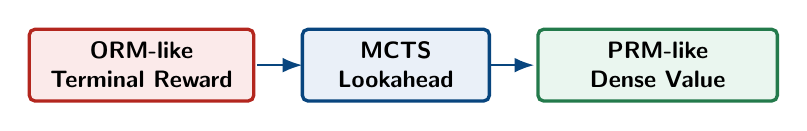
\begin{tikzpicture}[scale=0.95, transform shape]
\node[redbox, minimum width=3.0cm] at (0,0) {ORM-like\\Terminal Reward};
\node[bluebox, minimum width=2.5cm] at (3.4,0) {MCTS\\Lookahead};
\node[greenbox, minimum width=3.2cm] at (6.9,0) {PRM-like\\Dense Value};
\draw[arrow] (1.55,0) -- (2.15,0);
\draw[arrow] (4.65,0) -- (5.25,0);
\end{tikzpicture}
\end{center}

\vspace{0.6em}
\begin{block}{차별점}
\small
최종 결과만 보고 강화하는 것이 아니라, 미래 진단 value를 현재 검사 선택으로 되돌려 action-level supervision을 만든다.
\end{block}
\end{frame}

\end{document}
